\section{Participants}
\label{sec:participants}
Eligible participants are consenting adults able to understand the task, hear the guidance, view the scene with usual correction and safely use the seated setup and right controller. Handedness, visual correction and prior XR and voice-assistant experience are recorded. Sample size and the enrollment ceiling will be determined before recruitment by a power analysis for the theta-adjusted repeated-measures outcome that accounts for plausible within-participant variation and incomplete observations.


\section{Experiment Design}
\label{ch:methodology}
The user study uses a within-participant design to answer the research questions in Section~\ref{sec:research-questions}.

The study design draws on Chiossi et al.'s visual-search study, which combines search outcomes with eye-tracking measures~\cite{chiossi2024searching}. This study keeps that separation between task performance and visual behavior but changes the research question to voice identity, initially withholds the target identity, and uses a researcher-selected 25-second search limit. Complementary work by Pfeil et al. at UCF compares eye--head coordination in virtual and physical viewing~\cite{pfeil2018eyehead}. That work motivates retaining head motion alongside eye direction when interpreting gaze in this application.

\draftnote{This section specifies the proposed confirmatory procedure. The implemented snapshot supports one practice trial, two 40-trial blocks, and a final questionnaire handoff. It also records pre-cue starting geometry and balances target direction and height within each block. Sample size and pilot acceptance rules remain unresolved.}
\subsection{Voice Manipulation and Comparison Rationale}
This thesis compares two ways of personalizing assistance: a synthetic voice derived from the participant's recorded speech and a neutral voice selected by that participant from the supplied catalog. Letting participants choose the neutral alternative ties the comparison to a design choice a user could face. The within-participant task provides repeated observations under both configurations. Similarity ratings indicate whether participants heard the clone as resembling themselves, whereas performance and experience measures compare how each voice functions as guidance.

Gaze contingency and the agent's decision rules are common to both conditions. Because the target identity is initially hidden, participants receive repeated guidance in the assigned voice on every trial. The decision model, memory, and gaze awareness are held constant rather than varied as independent factors.

\subsection{Design and Trial Allocation}
The study uses a within-participant comparison of two voice conditions: a neutral voice and a self-similar synthetic voice. Both conditions use the same guidance policy, semantic phrase library, selection method and visual-feedback settings, although actual phrase sequences may differ because guidance responds to behavior. Because the neutral voice is chosen by the participant whereas the clone is derived from the participant's speech, the two voices may also differ in preference, gender presentation and synthesis quality. The contrast therefore cannot isolate self-similarity from these features.

A saved, balanced randomized allocation assigns neutral-first or self-similar-first order. Counterbalancing the order distributes possible carryover from the first block across the two voices~\cite{williams1949residual}, although it does not remove carryover. Each participant completes one practice trial followed by two measured blocks of 40 trials, one per voice. The practice trial uses the first voice in the assigned order (the self-similar voice for Order A, or the neutral voice for Order B) and is excluded from measured outcomes. A seed makes the trial schedule reproducible. Nominal horizontal-angle quotas are identical across blocks, with trial order and left/right assignments randomized subject to those quotas. Within each block, each bilateral angle category (45, 90 and 135 degrees) has four left and four right assignments.

\begin{table}[htbp]\centering
\caption[Study allocation]{Study allocation. Nominal wall angles are schedule categories, not exact object bearings or accumulated head rotation.}
\tagpdfsetup{table/header-rows={1}}
\begin{tabularx}{\linewidth}{@{}lX@{}}\toprule
Parameter & Allocation \\\midrule
Voice conditions & Neutral voice; self-similar synthetic voice \\
Measured trials & 40 per block; 80 per participant \\
Practice & One trial; excluded from outcomes \\
Absolute nominal wall step & Eight trials each at 0, 45, 90, 135 and 180 degrees per block \\
Vertical allocation & 20 targets above and 20 below readiness-cross height per block; four above and four below at each nominal angle \\
Condition order & Counterbalanced neutral-first and self-similar-first \\
Active search limit & 25 seconds, excluding explicit pauses \\
Selection & Right-controller ray and a trigger press \\\bottomrule
\end{tabularx}
\end{table}

Objects vary in position within each plane of the shared layout, so each trial specifies the exact starting angle and target height in addition to the assigned wall. Vertical allocation is defined by target-center height relative to the readiness cross rather than the participant's seated eye height. The cross is placed at the midpoint of the permitted object-height range, and each assigned target center lies between 10 and 45 percent of that range above or below it. The lower bound keeps every target clearly above or below the cross, and the upper bound keeps targets away from the floor and the top of the wall. Pilot sessions will assess target visibility and seated comfort at both extremes.

\begin{figure}[htbp]\centering
\IfFileExists{figures/study-procedure-current.pdf}{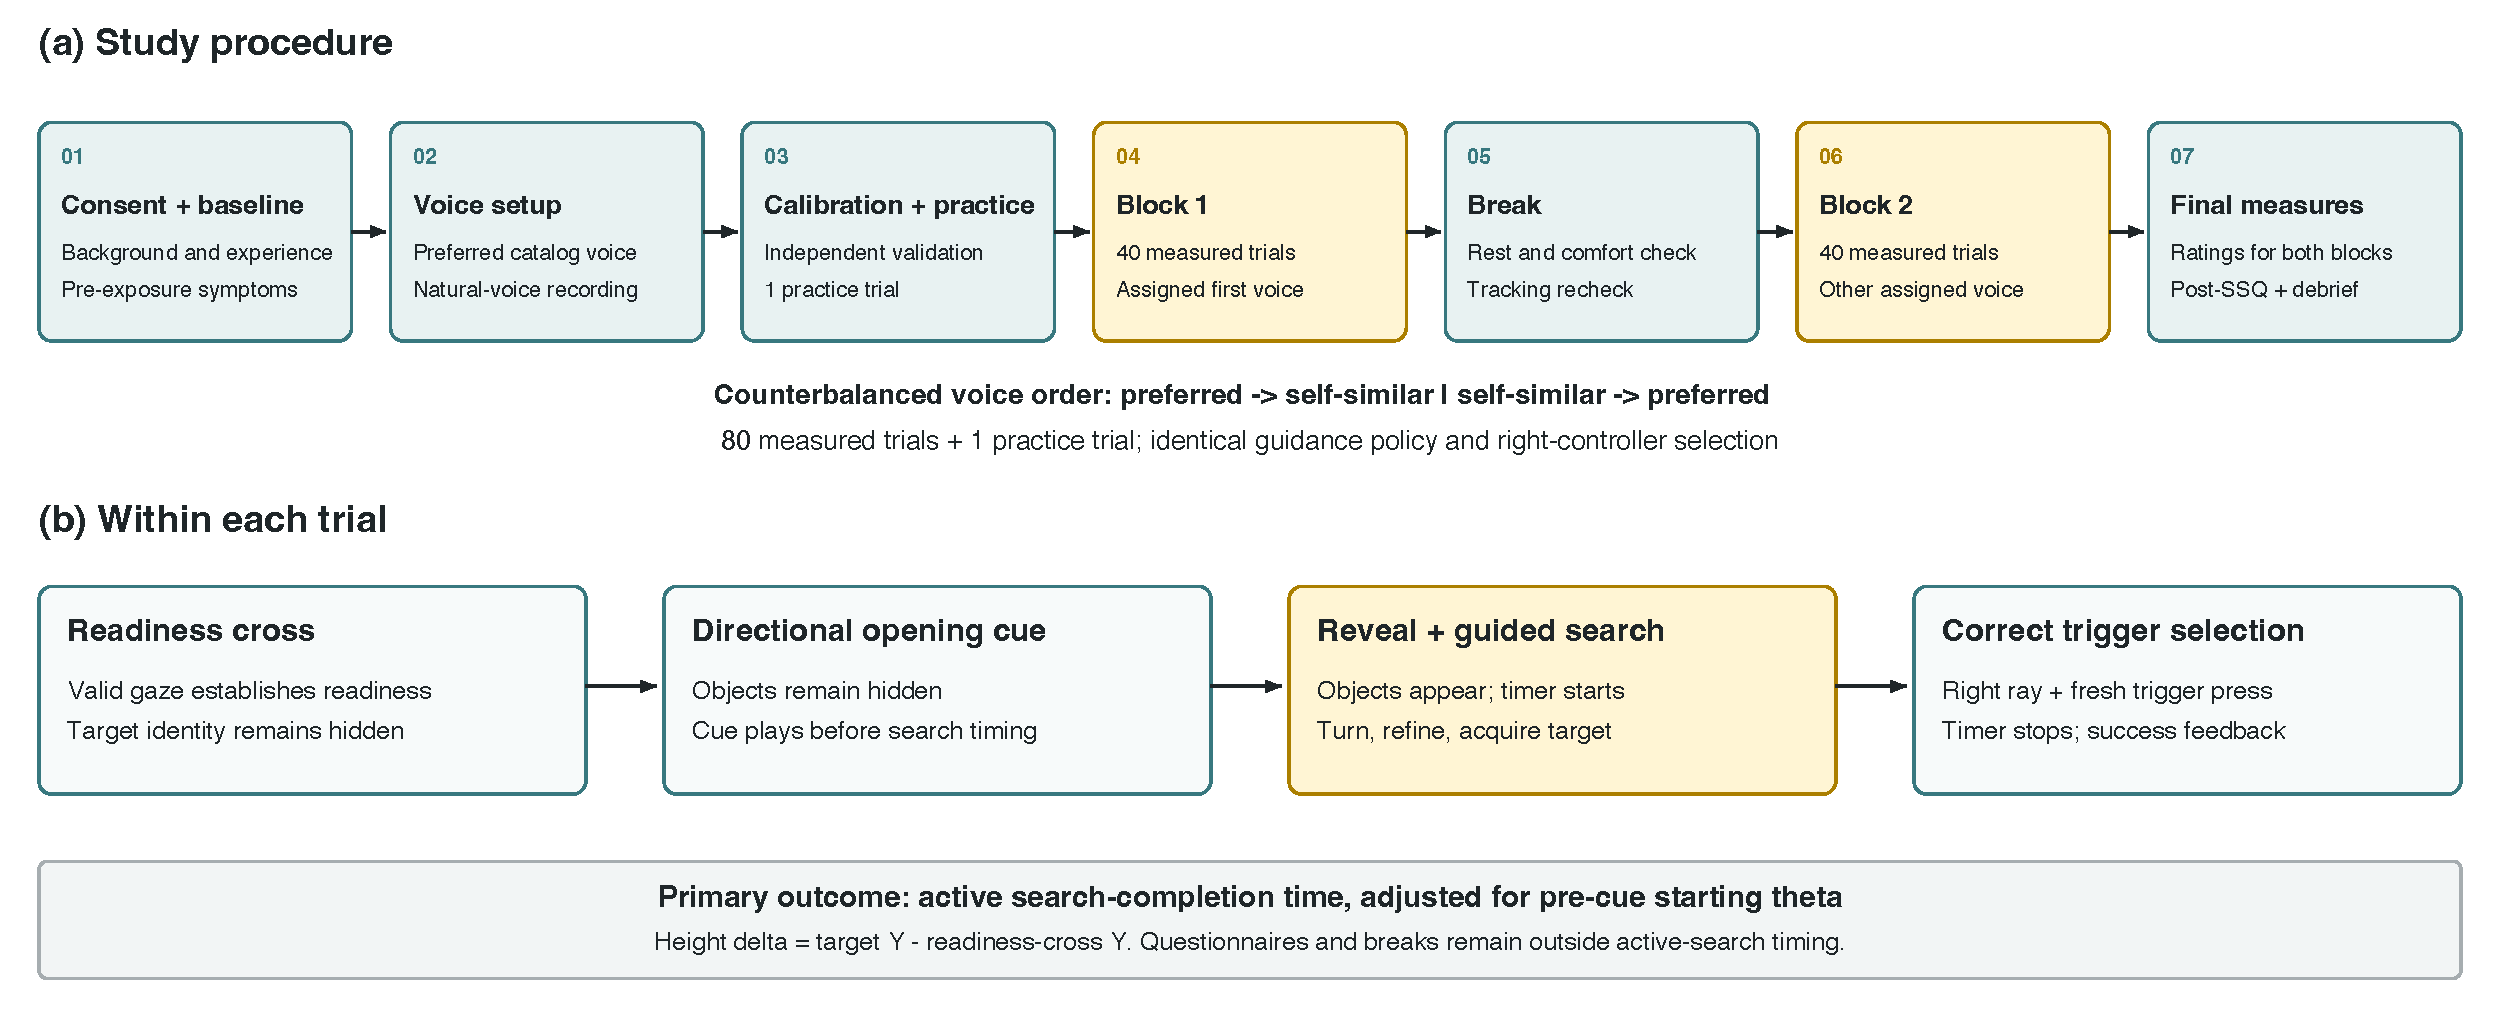
\includegraphics[width=\linewidth,alt={Consent, Selected Voice choice, audio intake and headset setup precede two counterbalanced orders. Order A runs a self-similar practice trial, a blue 40-trial self-similar block, a break and a gold 40-trial neutral block; Order B reverses the colors. Both end with a side-by-side final survey. Each trial separates readiness, opening cue, reveal and trigger selection.}]{figures/study-procedure-current.pdf}}{\fbox{\parbox{0.94\linewidth}{Consent $\rightarrow$ Selected Voice $\rightarrow$ audio intake $\rightarrow$ headset setup $\rightarrow$ practice $\rightarrow$ 40-trial voice block $\rightarrow$ break $\rightarrow$ 40-trial voice block $\rightarrow$ survey and debrief. Within each trial: readiness cross $\rightarrow$ opening cue $\rightarrow$ object reveal and active search $\rightarrow$ correct trigger selection.}}}
\caption[Study procedure and trial timing]{Study procedure and trial timing. (a) Shared setup precedes the two counterbalanced orders; color marks the voice heard in each block, blue for the self-similar voice and gold for the neutral voice. The practice trial uses the first assigned voice and is excluded from outcomes. (b) Opening guidance precedes object reveal; active completion time ends at correct right-trigger selection. The success path shown here is bounded by a 25-second active-search deadline; expiry ends the attempt without a successful completion time. Questionnaires and between-trial breaks remain outside active-search timing.}
\label{fig:study-procedure}
\end{figure}

\clearpage
Nominal angle steps are defined relative to the readiness (start) wall, which is the previous target wall. For the first measured trial, this reference is the practice target wall. The first measured cross is centered on its wall. Each later cross is shifted sideways by a seeded offset of up to 20 percent of the usable half-width. Target placement happens when readiness completes, while all objects remain hidden and before the opening cue. At that moment, the application rotates the horizontal bearing from the participant's eye origin to the cross by the assigned signed angle, places the target where that bearing meets the assigned wall, and arranges the remaining objects around it. The exact starting angle defined below therefore equals the assigned category at that instant. If the required position falls outside the wall, the session stops so the participant can recenter, rather than substituting a different angle or trial. Final positions depend on the saved eye origin as well as the seed, so each layout is reconstructed from the saved object positions.

\subsection{Research Questions and Outcomes}
Each research question in Section~\ref{sec:research-questions} maps onto specific outcomes. RQ1 uses active completion time as the primary outcome, with missed targets and perceived workload, measured with an adaptation of NASA-TLX~\cite{hart1988nasatlx}, as secondary outcomes. RQ2 uses the Index of Pupillary Activity~\cite{duchowski2018ipa}, fixation count, and saccade frequency, which remain exploratory until the eye-event detectors are validated on the headset. RQ3 uses the interest/enjoyment subscale of the Intrinsic Motivation Inventory (IMI)~\cite{ryan1982control,mcauley1989imi}, with the other three IMI subscales reported alongside it. Agent perception, eeriness, voice experience, reliance, search behavior, and variation in the voice contrast with starting angle are exploratory. The hypotheses are directional, favoring the self-similar voice, but the voice contrasts are tested two-sided so that an advantage for the neutral voice would also be detected. Repeated trials are treated as within-participant observations, not as independent participants.


\section{Procedure}
Participants perform an agent-guided object-search task while seated on a swivel chair, with multiple colored geometric objects scattered across eight surrounding vertical planes. Although the application knows the target identity, the participant does not receive a color-and-shape description before searching. Instead, the agent guides the participant toward the target wall and then refines the direction horizontally, vertically or diagonally. The participant selects an object using the right-controller ray and trigger. Looking at an object, receiving a gaze confirmation or pointing at it does not by itself complete the trial.

Each trial begins with the participant looking at a readiness cross. Once readiness is established, an opening directional cue plays while the objects remain hidden, and object reveal then starts active search timing. A correct trigger selection before the 25-second active-search deadline stops timing and produces success feedback. An incorrect selection is counted, and search continues within that same limit.

If the target has not been selected after 25 seconds of active search, the trial ends as a timeout. The application hides the objects, cancels pending spatial hints, and plays a prepared encouragement in the assigned voice, beginning with ``Time up,'' before presenting the next readiness cross. For example, the agent may say, ``Time up. Let's shake that round off and start the next.'' Separate wording introduces the block break or acknowledges the final trial. The same deadline and phrase set apply to both voice conditions and to the single practice trial. A timeout advances the scheduled attempt without adding a replacement. Explicit pauses suspend the clock, whereas tracking loss alone does not. The 25-second limit is a researcher-selected protocol parameter, not a threshold drawn from the cited studies.

Before participant use, consent materials will be updated to describe ElevenLabs transcription, cloning, and synthesis, including the data transmitted, retention, access, and deletion arrangements. After consent, participants audition the catalog voices, rate each one, and choose their Selected Voice; the neutral voice is chosen explicitly rather than inferred from participant gender. They then complete an audio intake survey. A generic intake agent, whose voice is outside the catalog and is never assigned to either condition, reads nine fixed questions: four eligibility questions (age, hearing, vision with usual correction, and ability to remain seated and use the right controller) and five background questions (VR and voice-assistant experience, prior eye tracking, handedness, and current visual correction). A tone marks when each answer should begin. Voice capture begins only after a signed-consent attestation is recorded. All nine questions, and the optional fallback reading when the answers are too short, are completed before the researcher reviews the four eligibility answers, so a negative or unclear answer stops screening rather than passing automatically. Only a positive review, together with at least 30 seconds of estimated speech and 50 transcribed words, permits the system to clone the participant's voice from the answers, prepare both voices' phrase libraries in the Trial Review application under the participant's study ID, and transfer them to the headset, where the participant confirms their study ID and condition order before starting. The intake questions and the fallback reading passage, used only when the answers do not reach that threshold, are reproduced in Appendix~\ref{app:instruments}.

The researcher fits the headset and conducts vendor calibration followed by independent spatial validation across relevant heights, wall boundaries, distances and head orientations. If an offset correction is introduced, the targets used to fit it are kept separate from those used for independent validation. Standardized instructions explain that participants rely on the agent to discover the target and use the right trigger to select it. Participants then complete the single practice trial and the two assigned 40-trial blocks.

No questionnaire interrupts the block sequence. Instead, the final survey presents every condition-specific item once, with two response columns side by side, labeled \emph{Selected Voice} and \emph{Self-Similar Voice}, so that participants compare the two agents directly while rating each one. Breaks are offered between trials and at the block boundary, and any necessary in-trial pause is logged immediately. Tracking is rechecked between blocks and after headset adjustment. After headset removal, participants complete the side-by-side retrospective ratings, comparative voice preference, and debrief. Participants may request a pause or stop, and symptoms or technical problems prompt researcher assessment.

Figure~\ref{fig:survey-scopes} distinguishes administration time from reference scope: both columns are completed in the final session, but each rating refers to the block in which that voice was heard.

\begin{figure}[htbp]
\centering
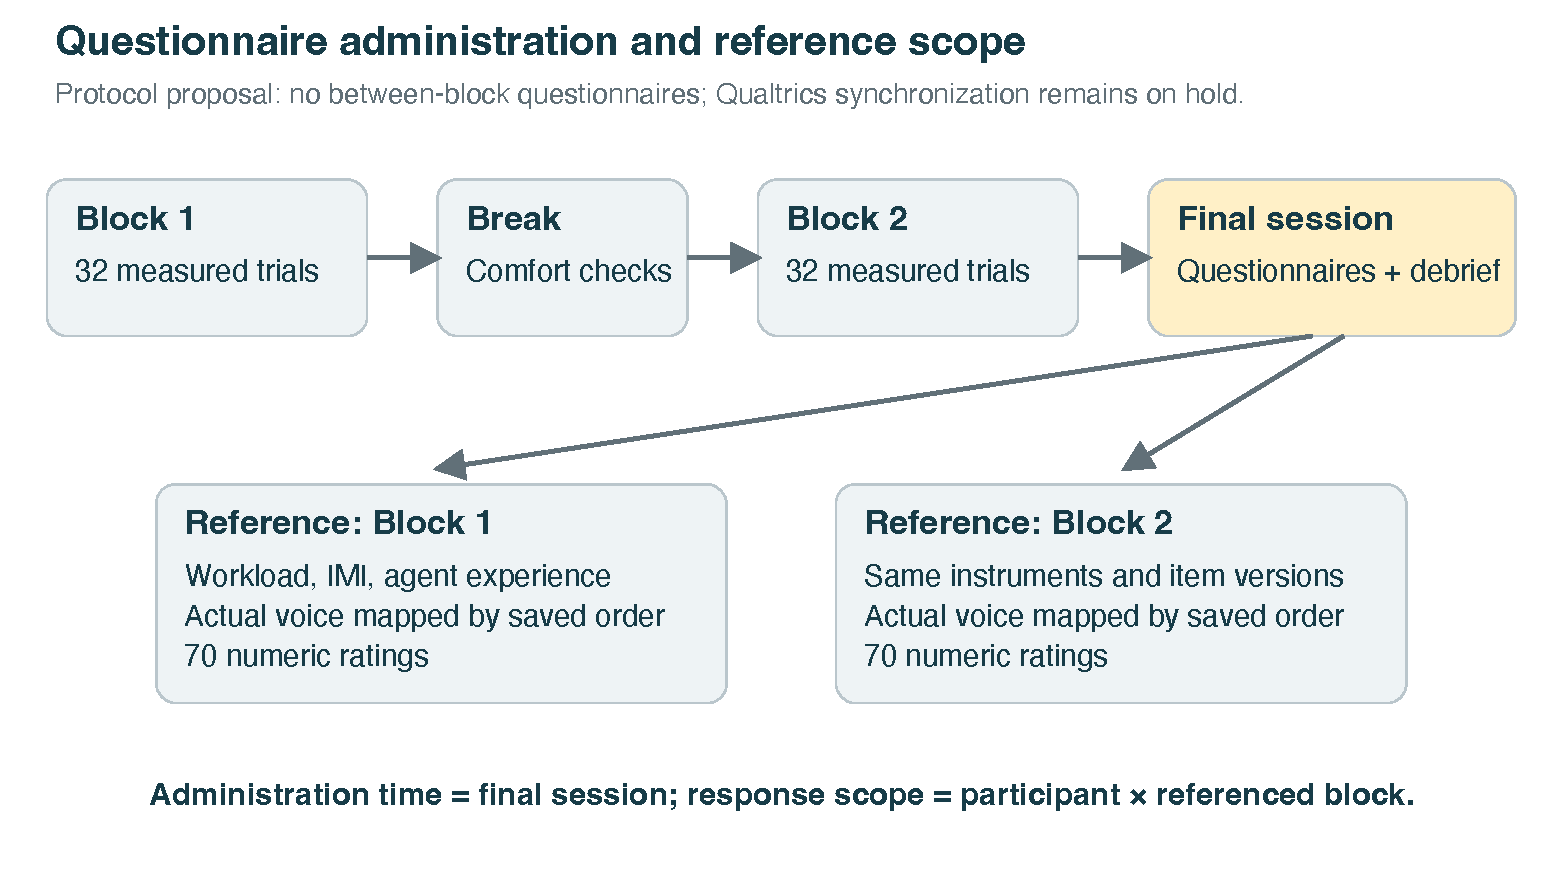
\includegraphics[width=\linewidth,alt={Two blocks separated by a break are followed by a final session with questionnaires referring separately to Block 1 and Block 2.}]{figures/survey-scopes.pdf}
\caption[Final questionnaire timing and block reference scope]{Proposed final retrospective administration. The intervening break contains comfort and tracking checks, not a block questionnaire. Each voice column contains 70 numeric ratings. The block in which each voice was heard is recovered from the saved counterbalanced order.}
\label{fig:survey-scopes}
\end{figure}


The survey columns name the two voices directly, as the Selected Voice and the Self-Similar Voice, so participants do not need to remember which block used which voice. Because the label identifies the self-similar condition, it may cue expectations about that voice; this tradeoff is noted as a limitation, and pilot sessions will check that participants understand both labels.

\subsection{Pilot Testing and Parameter Checks}
\label{sec:pilot}
Before confirmatory recruitment, pilot sessions verify the realized angle/height schedules, target visibility and seated comfort, readiness and selection behavior, gaze validity, audio timing and wording, and reconstruction of trial events from the saved data. Pilot assessment also measures survey comprehension and completion time. These checks inform calibration-acceptance, practice-proficiency and technical-stop criteria. The pilot also assesses whether the 25-second deadline is suitable, and the outcome is documented with the study build and questionnaire versions.
